
\begin{itemize}

\item Utilizando busqueda exacta

\begin{table}[H]
\centering
\renewcommand{\arraystretch}{1.2} 
\begin{tabular}{|c|c|c|c|c|c|}
\hline
\textbf{Iter} & \textbf{x$_{inicial}$} & \textbf{$x^k$} & \textbf{||$\nabla \mathbf{f(x^k)}$}|| & \textbf{f($\mathbf{x^k}$)}& \textbf{tiempo} \\
\hline
2  &  (0.24 , 0.85) &( 0.00000,0.00000 ) & 0.00000000 & -1.00000000 & 0.1553 \\
2  &  (0.09 , 0.43) &( 0.00000,0.00000 ) & 0.00000000 & -1.00000000 & 0.1578 \\
2  &  (0.85 , 0.12) &( -0.00000,-0.00000 ) & 0.00000000 & -1.00000000 & 0.1487 \\
2  &  (0.34 , 0.15) &( 0.00000,0.00000 ) & 0.00000000 & -1.00000000 & 0.2452 \\
2  &  (0.9 , 0.26) &( 0.00000,0.00000 ) & 0.00000000 & -1.00000000 & 0.1658 \\
2  &  (0.06 , 0.86) &( 0.00000,0.00000 ) & 0.00000000 & -1.00000000 & 0.2009 \\
2  &  (0.59 , 0.78) &( -0.00000,-0.00000 ) & 0.00000000 & -1.00000000 & 0.1500 \\
1  &  (1.9 , 5.49) &( 1.90000,5.49000 ) & 0.00000000 & -0.00000000 & 0.0000 \\
2  &  (1.29 , 2.26) &( -0.00000,-0.00000 ) & 0.00000000 & -1.00000000 & 0.1339 \\
1  &  (2.4 , 3.38) &( 2.40000,3.38000 ) & 0.00000029 & -0.00000003 & 0.0000 \\
1  &  (3.42 , 3.87) &( 3.42000,3.87000 ) & 0.00000000 & -0.00000000 & 0.0000 \\
2  &  (2.46 , 2.07) &( -0.00000,-0.00000 ) & 0.00000000 & -1.00000000 & 0.1129 \\
1  &  (5.65 , 6.18) &( 5.65000,6.18000 ) & 0.00000000 & -0.00000000 & 0.0000 \\
2  &  (2.46 , 2.18) &( 0.00000,0.00000 ) & 0.00000000 & -1.00000000 & 0.1028 \\
2  &  (1.28 , 1.49) &( -0.00000,-0.00000 ) & 0.00000000 & -1.00000000 & 0.2391 \\
2  &  (1.28 , 2.49) &( -0.00000,-0.00000 ) & 0.00000000 & -1.00000000 & 0.2502 \\
1  &  (3.78 , 2.62) &( 3.78000,2.62000 ) & 0.00000001 & -0.00000000 & 0.0010 \\
\hline
\end{tabular}
\end{table}


\begin{figure}
    \centering
    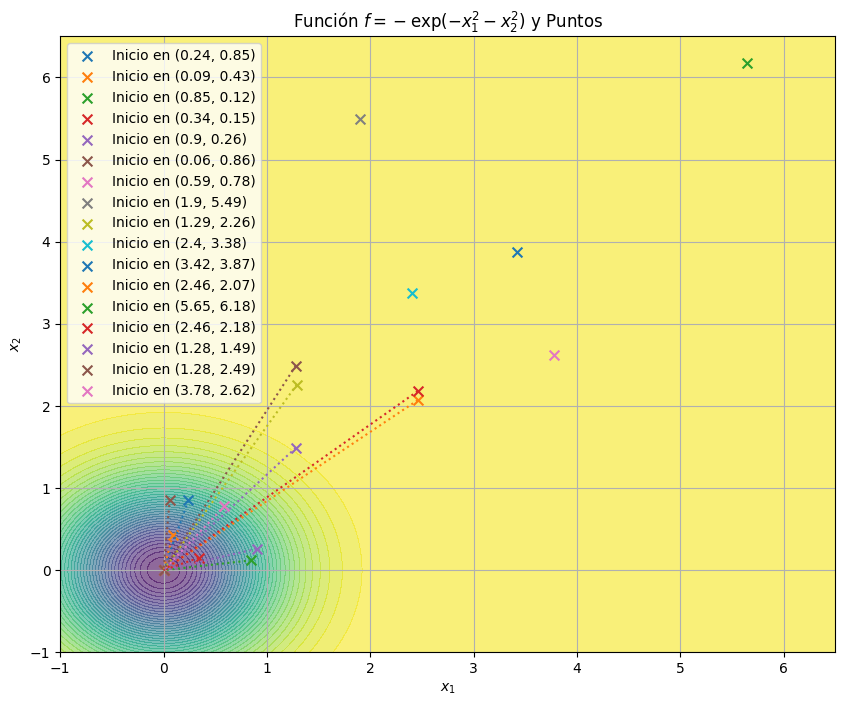
\includegraphics[width=0.65\linewidth]{figuras/PREG6_UNI.png}
    \label{fig:enter-label}
\end{figure}

\item Utilizando busqueda de Armijo


\begin{table}[H]
\centering
\renewcommand{\arraystretch}{1.2}
\begin{tabular}{|c|c|c|c|c|c|c|}
\hline
\textbf{Iter$_{total}$} & \textbf{Arm$_{total}$} &\textbf{x$_{inicial}$}& \textbf{$\mathbf{x^k}$} & \textbf{|| $\nabla$f($\mathbf{x^k}$) ||} & \textbf{f($\mathbf{x^k}$)}  & \textbf{tiempo} \\
\hline
16  &29 & (0.24 , 0.85) &( -0.00000,-0.00000 ) & 0.00000000 & -1.00000000 & 0.1175 \\
13  &23 & (0.09 , 0.43) &( -0.00000,-0.00000 ) & 0.00000000 & -1.00000000 & 0.1534 \\
12  &21 & (0.85 , 0.12) &( -0.00000,-0.00000 ) & 0.00000000 & -1.00000000 & 0.1336 \\
13  &23 & (0.34 , 0.15) &( -0.00000,-0.00000 ) & 0.00000000 & -1.00000000 & 0.1534 \\
16  &29 & (0.9 , 0.26) &( -0.00000,-0.00000 ) & 0.00000000 & -1.00000000 & 0.2129 \\
15  &27 & (0.06 , 0.86) &( -0.00000,-0.00000 ) & 0.00000000 & -1.00000000 & 0.2155 \\
16  &30 & (0.59 , 0.78) &( -0.00000,-0.00000 ) & 0.00000000 & -1.00000000 & 0.2456 \\
1  &0 & (1.9 , 5.49) &( 1.90000,5.49000 ) & 0.00000000 & -0.00000000 & 0.0000 \\
\hline
\end{tabular}
\end{table}

\begin{figure}
    \centering
    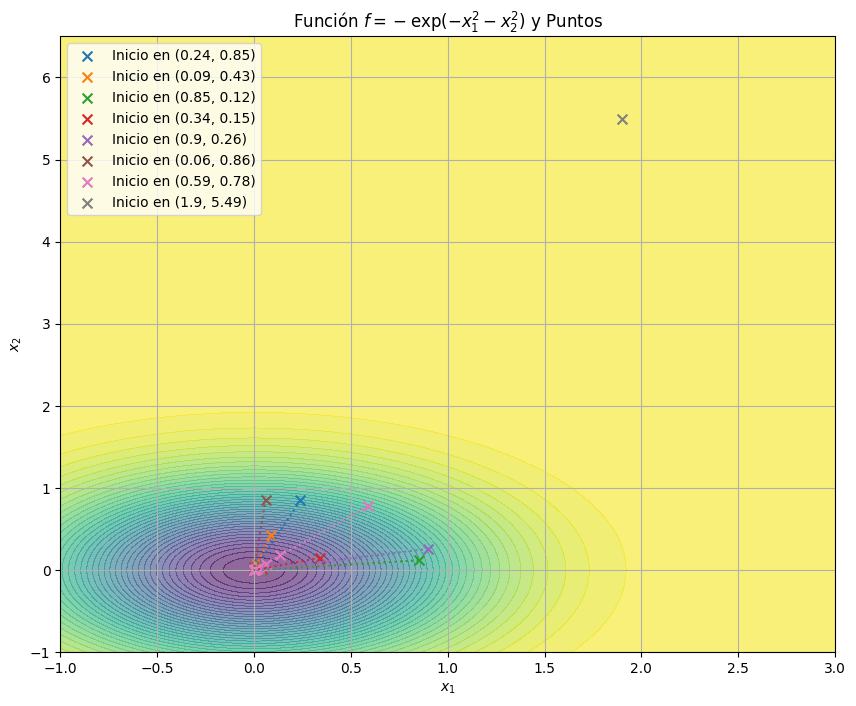
\includegraphics[width=0.65\linewidth]{figuras/PREG6_ARMIJO.png}
    \label{fig:enter-label}
\end{figure}

\end{itemize}




